\section{Технический проект}
\subsection{Общая характеристика организации решения задачи}

Этот проект направлен на разработку системы, которая использует нечеткие нейронные сети для распознавания объектов на основе цветовых характеристик. Система будет способна анализировать изображения и выделять объекты, соответствующие заданным цветовым параметрам.

Основная цель - создание эффективной и точной системы распознавания объектов. Задачи включают:

\begin{itemize}
\item Разработка алгоритма нечеткой нейронной сети;
\item Создание базы данных для обучения и тестирования системы;
\item Интеграция системы с камерами для реального времени обработки изображений.
\end{itemize}

\subsection{Обоснование выбора технологии проектирования}

Нечеткие нейронные сети сочетают принципы нечеткой логики и нейронных сетей, что позволяет системе обрабатывать нечеткие и неточные данные, характерные для реальных изображений.

\subsubsection{Описание используемых технологий и языков программирования}

В процессе разработки приложения используются программные средства и языки программирования. Каждое программное средство и каждый язык программирования применяется для круга задач, при решении которых они необходимы.

\subsubsection{Нечеткие нейронные сети}

Комбинация нечеткой логики и нейронных сетей позволяет системе обрабатывать нечеткие данные. Мы используем нечеткие нейронные сети для улучшения точности распознавания объектов по цветовым характеристикам, даже когда данные имеют шум или неточности.

\subsubsection{Машинное обучение}

Применение алгоритмов машинного обучения для анализа и классификации данных. В нашем случае, мы обучаем модель на большом наборе изображений, чтобы система могла эффективно распознавать и классифицировать объекты в реальном времени.

\subsubsection{Python и его библиотеки}

Python является предпочтительным языком программирования благодаря своей читаемости, простоте и обширной экосистеме библиотек, подходящих для работы с данными и машинным обучением:

\begin{itemize}
\item NumPy: Используется для эффективной работы с массивами и матрицами, что критично для обработки изображений и численных вычислений.
\item Pandas: Предоставляет удобные структуры данных для анализа и манипуляции данными.
\item Matplotlib/Seaborn: Библиотеки для визуализации данных, которые помогают в анализе результатов и представлении данных.
\item OpenCV: Открытая библиотека для работы с компьютерным зрением, которая может использоваться для предварительной обработки изображений.
\item TensorFlow/Keras: Популярные фреймворки для глубокого обучения, которые предоставляют инструменты для создания, обучения и тестирования нейронных сетей.
\item Scikit-learn: Библиотека для машинного обучения, предоставляющая различные алгоритмы классификации, регрессии и кластеризации.
\end{itemize}

\paragraph{Достоинства языка Python}

Использование Python и его библиотек для создания системы распознавания объектов имеет ряд преимуществ:

\begin{itemize}
\item Простота и читаемость: Python известен своим чистым и легко читаемым синтаксисом, что упрощает написание и поддержку кода. Это особенно важно в больших проектах и при работе в команде.
\item Богатая экосистема: Python обладает обширной экосистемой библиотек и фреймворков, которые значительно ускоряют разработку и предоставляют готовые решения для многих задач.
\item Поддержка сообщества: Огромное сообщество разработчиков Python постоянно обновляет и улучшает существующие библиотеки, а также создает новые, что делает язык всегда актуальным.
\item Гибкость: Python позволяет интегрировать различные технологии и подходы, такие как нечеткая логика и нейронные сети, что идеально подходит для нашей системы.
\item Мультипарадигменность: Python поддерживает различные стили программирования — объектно-ориентированный, процедурный и функциональный, что дает гибкость в выборе подхода к решению задач.
\item Открытый исходный код: Большинство библиотек Python доступны бесплатно и имеют открытый исходный код, что снижает затраты на разработку.
\item Интеграция с другими языками: Python может быть легко интегрирован с другими языками программирования, что позволяет использовать его в качестве "клея" для различных компонентов системы.
\item Масштабируемость: Python и его библиотеки подходят как для прототипирования, так и для масштабирования систем на производство.
\item Поддержка научных вычислений: Библиотеки, такие как NumPy и SciPy, предоставляют мощные инструменты для научных вычислений, что необходимо при обработке изображений и данных.
\item Визуализация данных: С помощью Matplotlib и Seaborn можно легко создавать графики и визуализации, что полезно для анализа данных и результатов системы.
\item Машинное обучение и глубокое обучение: TensorFlow, Keras и Scikit-learn предоставляют обширные возможности для создания, обучения и тестирования моделей машинного обучения и глубокого обучения.
\end{itemize}

Эти преимущества делают Python и его библиотеки идеальным выбором для разработки системы распознавания объектов, особенно когда требуется работа с большими объемами данных и сложными алгоритмами.

\paragraph{Недостатки языка Python}

\begin{itemize}
\item Несмотря на множество преимуществ Python, существуют и недостатки, которые следует учитывать при выборе языка для проекта:
\item Скорость выполнения: Python часто критикуют за его относительно медленную скорость выполнения по сравнению с компилируемыми языками, такими как C или C++. Это связано с его динамической типизацией и интерпретируемостью.
\item Потребление памяти: Программы на Python могут потреблять больше памяти, что может быть проблемой для систем с ограниченными ресурсами.
\item Мобильная разработка: Python не является идеальным выбором для мобильной разработки. Другие языки, такие как Swift и Kotlin, лучше подходят для создания мобильных приложений.
\item Встроенные ограничения: Python имеет некоторые встроенные ограничения, такие как Global Interpreter Lock (GIL), который может затруднять полноценное использование многоядерных процессоров в многопоточных программах.
\item Игровая разработка: Хотя существуют библиотеки для создания игр на Python, он не является основным выбором для профессиональной разработки игр, где предпочтение отдают таким языкам, как C++ или C\# .
\item Строгость типизации: Python использует динамическую типизацию, что может привести к ошибкам во время выполнения, которые были бы обнаружены на этапе компиляции в языках со строгой типизацией.
\item Базовые настройки и оптимизация: Для достижения максимальной производительности может потребоваться дополнительная работа по оптимизации и настройке, включая использование сторонних инструментов.
\item Зависимости: Управление зависимостями в Python может быть сложным, особенно когда проекты становятся большими и сложными.
\item Безопасность: Python имеет открытый исходный код, что может представлять определенные риски безопасности, если не принимать соответствующие меры.
\item Работа с базами данных: Взаимодействие с некоторыми базами данных может быть менее эффективным по сравнению с языками, специализированными на этом, например, SQL.
\end{itemize}

Эти недостатки не делают Python плохим выбором; скорее, они подчеркивают важность тщательного анализа требований проекта и возможных ограничений перед выбором инструментов для его реализации.

\subsection{Диаграмма компонентов}

Диаграмма компонентов представляет структуру системы в виде набора компонентов и их взаимосвязей. Каждый компонент отвечает за определенную функцию в рамках системы и может включать в себя подсистемы или модули.

\subsubsection{Структура компонентов}
На диаграмме компонентов изображены основные блоки системы, такие как:

\begin{itemize}
\item Графический интерфейс пользователя: Модуль, отвечающий за взаимодействие с пользователем, представление результатов и получение входных данных.
\item Модуль предварительной обработки данных: Отвечает за подготовку данных к анализу, включая фильтрацию шума и нормализацию изображений.
\item Модуль нечеткой нейронной сети: Ядро системы, реализующее алгоритмы обучения и распознавания объектов.
\item База данных: Хранит обучающий и тестовый наборы данных, а также результаты работы системы.
\item Модуль анализа данных: Производит анализ данных, классификацию и предоставляет статистику по результатам.
\end{itemize}

\subsubsection{Взаимодействие компонентов}
Компоненты системы взаимодействуют друг с другом следующим образом:

\begin{enumerate}
\item Пользователь загружает изображение через графический интерфейс пользователя.
\item Интерфейс передает изображение в модуль предварительной обработки данных.
\item После обработки данные передаются в модуль нечеткой нейронной сети для распознавания объектов.
\item Результаты распознавания сохраняются в базе данных.
\item Модуль анализа данных извлекает результаты из базы данных и представляет их пользователю через графический интерфейс пользователя.
\end{enumerate}

Диаграмма компонентов представленна на рисунке ~\ref{componentdiagram:image}.

\begin{figure}[ht]
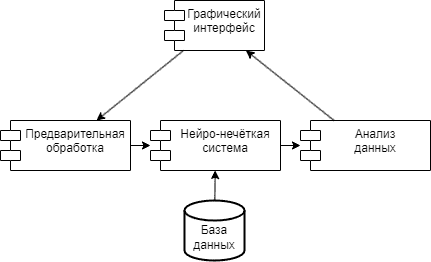
\includegraphics[width=1\linewidth]{componentdiagram}
\caption{Диаграмма компонентов системы}
\label{componentdiagram:image}
\end{figure}

\subsection{Содержание информационных блоков. Основные сущности}

Информационные блоки системы распознавания объектов представляют собой структурированные данные, которые используются для обучения, тестирования и работы системы. Основные сущности, которые являются частью этих блоков, включают:

\begin{itemize}
\item Изображение: Основной объект анализа, содержащий объекты для распознавания.
\item Объект: Целевая сущность на изображении, которую необходимо распознать и классифицировать.
\item Цветовой параметр: Характеристика объекта, используемая для его идентификации и классификации.
\item Метка класса: Определение категории, к которой принадлежит объект.
\item Набор данных: Коллекция изображений и соответствующих меток, используемых для обучения и тестирования системы.
\end{itemize}

Каждый информационный блок содержит данные, необходимые для выполнения специфических задач в рамках системы, таких как обучение нечеткой нейронной сети или классификация и анализ объектов. Структура информационных блоков разработана таким образом, чтобы обеспечить максимальную эффективность и точность при минимальных затратах времени на обработку данных.

\subsubsection{Структура информационного блока}

Каждый информационный блок состоит из следующих элементов:

\begin{enumerate}
\item Идентификатор изображения: Уникальный идентификатор, присваиваемый каждому изображению в базе данных.
\item Идентификатор объекта: Уникальный идентификатор, присваиваемый каждому распознанному объекту.
\item Цветовые характеристики: Набор параметров, описывающих цвет объекта в различных цветовых пространствах.
\item Геометрические параметры: Размеры и форма объекта, а также его положение на изображении.
\item Классификационные метки: Метки, указывающие на принадлежность объекта к определенной категории или классу.
\end{enumerate}

Эта структура позволяет системе быстро обрабатывать большие объемы данных и эффективно распознавать объекты с высокой степенью точности.

\subsubsection{Взаимодействие информационных блоков с компонентами системы}

Информационные блоки взаимодействуют с различными компонентами системы следующим образом:

\begin{enumerate}
\item Модуль предварительной обработки данных: Извлекает необходимые параметры из изображений и формирует информационные блоки.
\item Модуль нечеткой нейронной сети: Использует информационные блоки для обучения и классификации объектов.
\item База данных: Хранит информационные блоки и обеспечивает их доступность для других компонентов системы.
\item Модуль анализа данных: Производит дополнительный анализ информационных блоков для генерации отчетов и статистики.
\end{enumerate}

Таким образом, информационные блоки являются ключевым элементом системы, обеспечивающим ее функционирование и достижение поставленных целей.



